\documentclass[journal]{IEEEtran}

\usepackage{fancyhdr}
\usepackage{lastpage}
\usepackage{graphicx}
\usepackage[section]{placeins} %forces figures to appear in section
\usepackage{enumerate}
\usepackage{tikz}
\usepackage{ctable}
\usepackage{float}
\restylefloat{table}


% \usepackage{amsmath}
\usepackage[cmex10]{amsmath}
\interdisplaylinepenalty=2500
\usepackage{amsthm}
\usepackage{amsfonts}
\usepackage{bbm}
\usepackage{pgfplots}
\usepackage{hyperref}
\usepackage{url}
\usepackage[linewidth=1pt]{mdframed}
\floatstyle{plaintop}
\restylefloat{table}

%\bibliographystyle{IEEEtran}
\def\reals{\mathbb{R}}

% correct bad hyphenation here
\hyphenation{op-tical net-works semi-conduc-tor}


\begin{document}

\title{Guidance and Path Planning of a Parallel Robot without Visual Feedback}

\author{Thomas~Rochais$^*$,
        Courtney~Sheyko,
        and~Farhad~Jafari~% <-this % stops a space

\thanks{Thomas Rochais is a graduate student at the University of Pennsylvania in the Department of Physics and Astronomy, Philadelphia, PA, 19104 USA e-mail: thb@sas.upenn.edu.}% <-this % stops a space
\thanks{Courtney Sheyko is a recent graduate from the Department
of Mathematics at the University of Wyoming, Laramie,
WY, 82070 USA e-mail: courtneygrace1290@gmail.com.}% <-this % stops a space
\thanks{Farhad Jafari is a faculty member in the Department
of Mathematics at the University of Wyoming, Laramie,
WY, 82070 USA e-mail: fjafari@uwyo.edu.}
\thanks{$^*$Corresponding author}}


% The paper headers
\markboth{Journal of \LaTeX\ Class Files,~Vol.~?, No.~?, October~2017}%
{Shell \MakeLowercase{\textit{et al.}}: Bare Demo of IEEEtran.cls for Journals}

% make the title area
\maketitle

% As a general rule, do not put math, special symbols or citations
% in the abstract or keywords.
\begin{abstract}
Optimal path planning and design is a fundamental and deep question in many areas of science and engineering. Here, we explore a bumper-car feedback approach to path planning and design. We describe the kinematics of a model parallel robot having contact with the surface and develop a path planning strategy guided by the robot bumping into the walls. Using a Snell's law model for reflection from the wall, a model for the local curvature (derivable from the tangent space) of the wall is developed, and the robot is guided by feedback. Such a model would be important in guiding a rescue robot through a circuitous dust filled mine shaft, where visibility/sensor feedback is not an option. This design is coded in Matlab and simulations are run to show the resulting dynamics. The effect of robot geometries on the path design is investigated.
\end{abstract}

\section{Introduction}

\IEEEPARstart{T}{here} has been much research performed in path planning and design, robotics, and feedback dating back to 1970s and earlier. However, feedback through hitting boundary walls appears to be novel. Here we use feedback to advance a parallel robot on an unknown surface with boundary. As an example, the model we develop could be used to guide a rescue robot through a circuitous mine shaft where visibility/sensor feedback is not an option. Indeed, the robot could bounce off some obstacles as well as the boundaries of the mine shaft. The feedback from bounces could then be used to map the surrounding area and compute an optimal path strategy. Isafiade et al. \cite{Isafiade13} studied several path planning strategies for robots in underground terrains, but heavily relied on visual feedback. Also Gao et al. \cite{Gao13} used an approach to guide robots based on sonars. Futhermore, Naidoo et al. \cite{Naidoo15} proposed to use multiple robots working together for a rescue mission.

Another possible use would be for surgical robots where it might be impractical to add extra sensors, such as cameras or sonars on top of the robot. Burgner-Kahrs et al. \cite{Burgner15} discuss some of the difficulties involved in minimally invasive surgery for sites of difficult access. As one of the `three grand challenges' they mention the importance of shape and force sensing. They state that external cameras require line of sight with the robot, which is not possible in minimally invasive surgeries, and EM tracking requires an environment without any magnetic objects that could interfere with the magnetic field and decrease accuracy. Thus a robot without those constraints would be placed at a great advantage. Another study by Bergels et al. \cite{Bergeles15} uses concentric tube robots. However in this design stiffness in bending needed to be monitored as well as the need for multiple curved robot sections in order to navigate properly.

For simplicity, this paper only focuses on a spherical robot throughout. However it can be shown that any smoothly bounded convex robot diffeomorphic to a Euclidean ball would follow similar dynamics through a change-of-variable. As a result, our model is not as limited as it might first appear and can apply to much more than just a spherical robot.  

Since this project deals with robots both sliding and rolling on a surface, it falls into the category of non-holonomic constraints on the behavior of the robotic system. These constraints arise in systems such as wheeled mobile robots where rolling contact is involved as well as where angular momentum is conserved. Some of the theory for non-holonomic systems has been described by Vershik and Gershkovic in \cite{Vershik88}, and by Vidyasagar \cite{Vidyasagar02}, and it uses a combination of differential geometry, Lie algebras, control theory and non-linear systems of differential equations. 

In Section 1 we will present the assumptions made as well as introduce the notation and define some of the important terms. The reader is referred to Murray, Li, and Sastry \cite{book} for the notation and definitions used in this article. In Section 2, we will describe the derivations in our model. Finally, in Section 3, we will describe the code and present and discuss the results of simulations. In the appendix, we provide extra details for the kinetic derivations.

\section{Assumptions and Definitions}

For all surfaces $S$ on which the robot is allowed to roll, $S$ is assumed to be regular. That is, for each point $p \in S$ there exists a neighborhood $V \subset \mathbb{R}^3$, an open set $U \subset \mathbb{R}^2$, and a map $c : U \rightarrow V \cap S$. Our local coordinate chart, $c$, is assumed to be twice differentiable and a homeomorphism from $U$ to $V \cap S$ (i.e. $c$ is continuous, bijective and has a continuous inverse). Moreover, we 
%define $\alpha$ as the inverse of $c$ 
assume that for every $ \alpha = (u,v) \in U$, the map $\frac{\partial c}{\partial \alpha}: \mathbb{R}^2 \rightarrow \mathbb{R}^3$ is injective. The surface on which the robot is rolling is assumed to have perpendicular "walls" as its boundaries. As the robot rolls on the surface, the shape and the surface of the robot are limited such that there is only one `theoretical' contact point between the robot and the surface unless a boundary is hit, in which case only two `theoretical' contact points are allowed. However, due to the discretization of the surfaces used in our model a few more nearby contact points are actually allowed. Please see the description of the code for details on how many points are allowed and how to modify this within the code.

Figure 1, provides a visualization of the spherical robot on the surface. In particular, the robot's reference frame is named `F' (or sometimes `f') and the surface's reference frame is named `O' (or sometimes `o'). Then, $\rho$ (or sometimes just `r' in the code) refers to the radius of the spherical robot, $\omega_x,\omega_y,\omega_z$ refer to the rolling velocities, and $v_x,v_y$ refer to the sliding velocities in the reference frame of the robot. Table 1 further describes the symbols used and their meaning.

\begin{figure}
\centering
\hspace{0cm}
    \includegraphics[width=3.5in]{Sphere_45.eps}
    \vspace{0cm}
    \caption{Variables and Mapping.}
    \label{fig:sim}
\end{figure}

 \begin{table}[htp]

\caption{ Variables}

\centering
\begin{tabular}{ll}
\\
\hline
\hline
Symbols & Description\\
\hline
o & Refers to the frame of the surface\\
f & Refers to the frame of the robot\\
C & Refers to contact frames\\
L & Refers to local frames\\
$c$ & Local coordinate chart\\
  & \ \ $(u,v) \in \mathbb{R}^2 \rightarrow (x,y,z) \in \mathbb{R}^3$\\
$c_u$,$c_v$ & Partial derivatives of $c$\\
$c^T$ & Transpose of $c$\\
%$\alpha$ & Inverse of $c$\\
%$\dot{\alpha}$ & Refers to the time derivative of $\alpha$\\
$\psi$   & The angle of contact between the \\
  & \ \ tangent vectors $\frac{\partial c_f}{\partial u_f}$ and $\frac{\partial c_o}{\partial u_o}$\\
$v_x,v_y,v_z$ & Linear velocities\\
$\omega_x,\omega_y,\omega_z$ & Rolling velocities\\
$V_{ab}$ & Body velocity vector of frame b \\
  & \ \ with respect to frame a\\
$\rho$ & Radius of spherical robot\\
M & Metric tensor\\
K & Curvature tensor\\
T & Torsion form\\
$\hat{a}$ & Short notation where $\hat{a}b = a \times b$\\
$Ad_g~A$  & Adjoint transformation of A\\
\hline
\hline
\end{tabular}
\end{table}

Furthermore, $M_p, K_p,$ and $T_p$ are referred to as geometric parameters of the surface where $M_p$ is defined as the metric tensor, $K_p$ is the curvature tensor of the surface, and $T_p$ is the torsion form of the surface.  Specifically, $M_p$ satisfies:
\begin{center}
Equations 1:
\end{center}

\[I_p = M_p \cdot M_p\]
where


\[I_p = 
\left[
\begin{array}{c c}
c_u^T c_u & c_u^T c_v \\
c_v^T c_u & c_v^T c_v \\
\end{array}
\right].
\]


Also, if we let
\[N(u,v) = \frac{c_u \times c_v}{|c_u \times c_v|} = n,\]
then the second fundamental form for the surface is:

\[II_p = 
\left[
\begin{array}{c c}
c_u^T n_u & c_u^T n_v \\
c_v^T n_u & c_v^T n_v \\
\end{array}
\right],
\]
and thus the curvature tensor for the surface is

\[K_p = M_p^{-T}II_pM_p^{-1}.\]

Finally, the torsion form is given by:

\[T_p = 
\left[
\frac{c_v^T c_{uu}}{||c_u||^2||c_v||} ~~ \frac{c_v^T c_{uv}}{||c_u||~||c_v||^2}
\right].\]

\section{Model}

\subsection{Generalized contact kinematics}
After some computations we can derive a system of equations which describes the contact kinematics of the robot as it moves along the surface. Appendix A shows the general derivations for the case of both sliding and rolling robot. However, we mainly focus on the robot rolling without sliding, and this special case can be described by the following system:
\begin{center}
Equations 2:
\end{center}


\[
\left[
\begin{array}{c}
\dot{u_f}\\
\dot{v_f}\\
\end{array}
\right]
= M_f^{-1}(K_f + R_{\psi} K_o R_{\psi})^{-1}
\left[
\begin{array}{c}
-\omega_y\\
\omega_x\\
\end{array}
\right]
\]



\[
\left[
\begin{array}{c}
\dot{u_o}\\
\dot{v_o}\\
\end{array}
\right]
= M_o^{-1}R_{\psi}(K_f + R_{\psi} K_o R_{\psi})^{-1}
\left[
\begin{array}{c}
-\omega_y\\
\omega_x\\
\end{array}
\right]
\]


\[
\dot{\psi} =  T_f M_f 
\left[
\begin{array}{c}
\dot{u_f}\\
\dot{v_f}\\
\end{array}
\right]
+ T_o M_o
\left[
\begin{array}{c}
\dot{u_o}\\
\dot{v_o}\\
\end{array}
\right] \]
These equations also appear in (\cite{book}, pages 332-345).  In our model we define $c_f$ as follows:
\begin{center}
Equation 3:
\end{center}


\[ c_f(u_f,v_f)=
\left[
\begin{array}{c}
\rho \cos{u_f} \cos{v_f}\\
\rho \cos{u_f} \sin{v_f}\\
\rho \sin{u_f} +1\\
\end{array}
\right],\]

where $- \pi/2 < u_f < \pi/2$ and $- \pi < v_f < \pi$ and $\rho$ is the radius of the sphere. For simplicity, the robot and surface are defined so that the initial contact point is at the origin.


\subsection{Change of coordinates}
Unfortunately, the above system of equations is not convenient to deal with when trying to directly input the velocity of the robot (`F' reference frame) with respect to the surface (`O' reference frame) rather than the contact velocities whose reference frames vary with the contact point. As a result we make a change of coordinates for the velocities. After performing the derivations from Murray, Li, and Sastry \cite{book} we are able provide here our final results:
\begin{center}
Equations 4:
\end{center}
%\begin{mdframed}[leftmargin=10pt,rightmargin=10pt]
\begin{center}
	$V_{l_ol_f} = (I-Ad^{-2}_{g_{fc_f}}) V_{oc_f} + Ad^{-1}_{g_{fc_f}}V_{of}$ \\
\end{center}
where we have the following:


\begin{align*}
Ad_{g_{fc_f}} &= \begin{bmatrix}
		R_{fc_f} & \hat{p}_{fc_f} R_{fc_f} \\
		0 & R_{fc_f}
              \end{bmatrix} \\ \\
R_{fc_f} &= \left[ \frac{c_u}{||c_u||}, \frac{c_v}{||c_v||}, \frac{c_u\times c_v}{||c_u\times c_v||}  \right] \\ \\
c_u &= \frac{\partial c_f}{\partial u_f} \\ \\
c_v &= \frac{\partial c_f}{\partial v_f}\\ \\
p_{fc_f} &= c_f(\alpha_f(t)) = c_f(u_f(t), v_f(t)) \\ \\
V_{oc_f} &=  \begin{bmatrix}
				R_{c_oc_f} & 0 \\
				0 & R_{c_oc_f}
			\end{bmatrix}
			V_{oc_o} +  \begin{bmatrix}
							0 \\
							0 \\
							0 \\
							0 \\
							0 \\
							\dot{\psi}
						\end{bmatrix} \\ \\
V_{oc_o} &=  \begin{bmatrix}
				M_o\dot{\alpha}_o \\
				0 \\
				-(0,1)\cdot(K_oM_o\dot{\alpha}_o) \\
				(1,0)\cdot(K_oM_o\dot{\alpha}_o) \\
				T_oM_o\dot{\alpha}_o
			\end{bmatrix} \\ \\
R_{c_oc_f} &= \begin{bmatrix}
				cos(\psi) & -sin(\psi) & 0 \\
				-sin(\psi) & -cos(\psi) & 0 \\
				0 & 0 & 1
			 \end{bmatrix} \\ \\
V_{l_ol_f} &= \begin{bmatrix}
				v_x \\
				v_y \\
				v_z \\
				\omega_x \\
				\omega_y \\
				\omega_z \\
			 \end{bmatrix}.
\end{align*}
%\end{mdframed}

\section{Implementation of the Model}
A Matlab code is developed to simulate the motion of the robot on different surfaces according to the above described kinematics. In short, the program solves for the velocity vector of equations 4 by solving the system of equations 2 after the change of coordinates prescribed in the previous section. This code is quite long (24 pages in total). A URL to this code is given here: 
\url{https://github.com/cbenn/guidancerobotics}

Here we describe the code which simulates a spherical robot rolling on a surface, using contact as its only way of guidance. The reader should refer to the section on assumptions for restrictions on the surface type. First, we describe the main program `Robotics.m', then a section is dedicated for each of its subroutines and a discussion of how the surfaces are generated. The results section describes the motion in a few example surfaces. 

\subsection{Storing the robot and the workspace}
The robot, the surface, and the workspace are read from folders storing an $n \times n$ black and white `.png' files, and then stored by the program into $n\times n\times n$ 3-dimensional matrices. The white (or 1 values) correspond to the object, while the black (0 values) correspond to empty space. The robot is stored into the `ROBOT' matrix, while the surface and the walls are combined into the `WORKSPACE' matrix. One can either enter the surface and walls separately or enter a full workspace containing both at once. Either way, the combined surface and walls are stored into the same `WORKSPACE' matrix.

\subsection{Robotics.m}
This is the main code. Everything is controlled by this script, which makes use of a few other functions described in the following sections.

\subsubsection{Loading the needed data into matrices}
At first the user is asked to choose a folder from which to load the robot and workspace. For simplicity of the code, this folder must be located in the local directory. Also, the folders must have the form `Bitmaps\_n' where $n$ is the size of the 3-dimensional WORKSPACE matrix which stores the workspace. Then the user has the option to choose between uploading the workspace all at once or the surface and walls separately. Those are uploaded and stored into the WORKSPACE matrix as the user selects them. Afterwards, the robot stored into 'Bitmaps\_n/Sphere\_robot/' is uploaded into the ROBOT matrix. For simplicity, the uploaded robot is set to have it's lowest point located at the coordinates (n/2,n/2,0) with respect to the workspace. Thus, after being uploaded it is shifted to match a proper location on the uploaded surface.
\subsubsection{Setting up the initial conditions}
The initial coordinates in both the workspace and the robot reference frames are then initialized. The user is also asked to enter a final time for the robot to roll as well as angular velocities $w_x$ and $w_y$. The other velocities ($w_z$, $v_x$, $v_y$, and $v_z$) are simply set to $0$, since we are only concerned about the robot rolling on the surface without sliding. The physical interpretation of those variables is that if we scale the radius of the robot to be $1$ unit of arbitrary [distance] and the final time to be $1$ unit of arbitrary [time], then the angular velocities have units of [rad/time] and the linear velocities have units of [distance/time]. Finally, using the known properties of the spherical robot, some matrices used in the contact equations are initialized right away.
\subsubsection{Rolling}
Then the robot is left to roll until the `current\_time' reaches `t\_final'. This is the first loop. Within that loop, we have the second loop which let's the robot roll until a boundary is hit. At each time step the surface is approximated to that of a plane using the `Get\_slopes.m' function. Then a new contact point is computed using the `Get\_bigZ\_bigC.m' and the `Get\_hit\_cont\_pts.m' functions. Furthermore, the program checks whether a boundary was hit using the output from `Get\_hit\_cont\_pts.m'. The same process repeats until a boundary is hit. When that happens, the code jumps out of the second loop.
\subsubsection{Bouncing and Reorientating}
After hitting a boundary, the code searches within $r/10$ to compute a normal and tangents to the wall at the point where the boundary was hit. Then using Snell's law, the bouncing angle is computed. This angle is converted into angular velocities, assuming no loss of kinetic energy. The robot is left to roll in the new bouncing direction for `$move$' number of time steps, where we currently have $move = r/5$. Afterwards, using the previously computed tangent vectors to the wall, the robot is reoriented into a direction parallel to that of the tangent plane to the wall, at the point where the boundary was hit. This is done by adjusting the angular velocities. Finally, the program loops back to the beginning of the first loop to repeat the same process over again.
\subsubsection{Plotting}
At last, when the final time is reached, several plots are output showing the path of the robot on the surface as well as a plot of the contact coordinates as a function of time.
\subsection{Getting the large computation matrices}
The `Get\_bigZ\_bigC.m' code is straight forward computationally, but has all the math hidden in it. The computed matrices bigZ and bigC are such that $bigZ \cdot \dot{c_{sol}} = bigC$ The derivations to obtain those matrices follow from the change of coordinates between the real velocities $V_{of}$ and the contact velocities $V_{l_ol_f}$.
%described in the change of coordinates section, and equation (5.28) of A Mathematical Introduction to Robotic Manipulation, by Murray, Li, and Sastry. 
Once those matrices are derived, the main `Robotics.m' code can use Euler's approximation method: 
\begin{center}
Equation 5:
\end{center}

  \begin{center}
    $c_{sol}(t+1) = \Delta t \cdot \dot{c_{sol}} + c_{sol}(t) = \Delta t \cdot bigZ^{-1} \cdot bigC + c_{sol}(t)$
  \end{center}
\subsection{Getting the contact points}
The purpose of the `Get\_hit\_cont\_pts.m' function is to find the new contact point with the surface after the robot has moved according to the contact equations. Furthermore, it looks for any contact point with the boundary: the hit\_pt. Due to the discretization of the robot, surface, and walls, several matches between the robot and the workspace are at first allowed, with a maximum spacing of $delta = r/10$. If two matches are a distance greater than $delta$ apart then they are considered to be part of two different physical contact points. If more than two physical contact points are found then the program terminates, since the contact equations do not allow for more than one contact point with the surface and one contact point with the walls. If only one contact point is found, then it is taken to be the new contact point between the robot and the surface. If there are exactly two contact points then the closest to the previous contact is the new contact point while the second one is the hit\_pt, i.e. the point of contact with the boundary. Finally, if there is no contact point found between the robot and the workspace, contact has been lost. This arises in the case where Euler's approximation was not good enough, or approximation of the surface to that of plane was too inaccurate. To make up for that, the robot is shifted in the x, y, and z directions by up to $delta\_move = round(r/10)$ until a contact point can be found. If after that no contact point is found the program terminates.
\subsection{Getting the partial derivatives}
The `Get\_slopes.m' program uses the contact point between the robot and the surface and looks at nearby points (up to $r/5$ away) to determine the partial derivatives $z_x$ and $z_y$ to the surface, at that particular contact point. Unfortunately, due to the discrete nature of the surface, the program might erroneously find an infinite partial derivative. In this case, the partial derivative is reset to its previously found value. Thus, the robot rolls on as if there were no change in the partial derivative. Those partial derivatives are returned, and can be used by the main code to approximate the local surface to that of a plane.
\subsection{Generating surfaces}
Surfaces can be generated using the Bitmaps.m code found in each `Bitmaps\_n' folder. There, the spherical robot is generated as well as a few sample surfaces. These objects are saved as n 2-dimensional $n\times n$ images (slices) into different folders. The variable `$n$' is the size of the 3-dimensional matrices which will store the robot and the workspace. The variable `$size\_workspace$' is a measure of the physical size of the workspace and is defined as $size\_workspace = n/r$ where $r$ is the radius of the spherical robot. Finally, new surfaces and walls can easily be generated by defining them in their parametric form: $(X,Y,Z) = (f(s,t),g(s,t),h(s,t))$.

\section{Results and Discussion}

\begin{figure}
\centering
    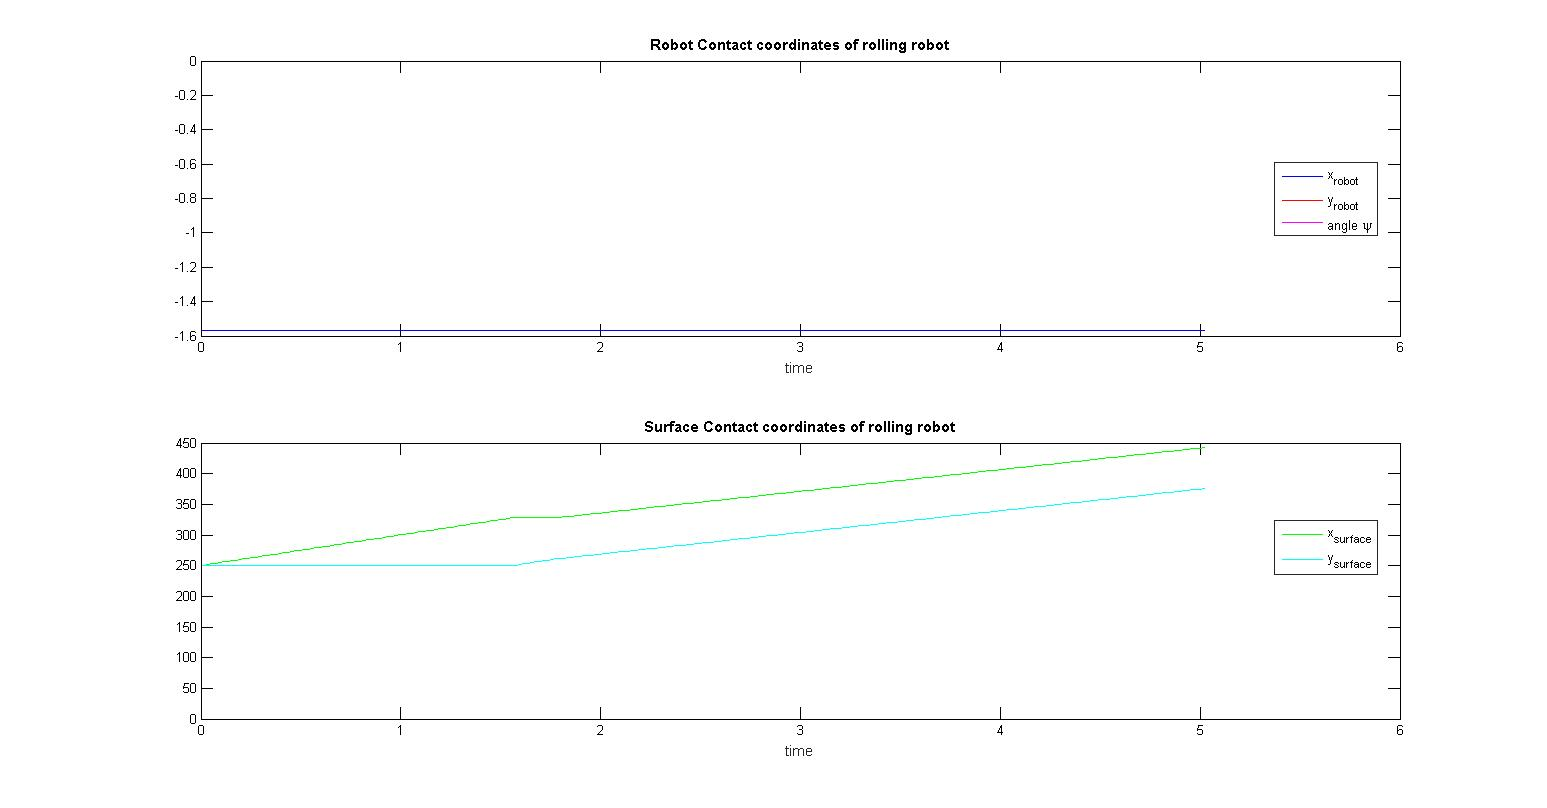
\includegraphics[width=3.5in]{flatsurf_2D.eps}
    \caption{Evolution of the contact coordinates as a function of time. The robot is rolling on a flat surface bounded by straight walls (see figure 3).}
    \label{fig:flatsurf2D}
\end{figure}
\begin{figure}
\centering
    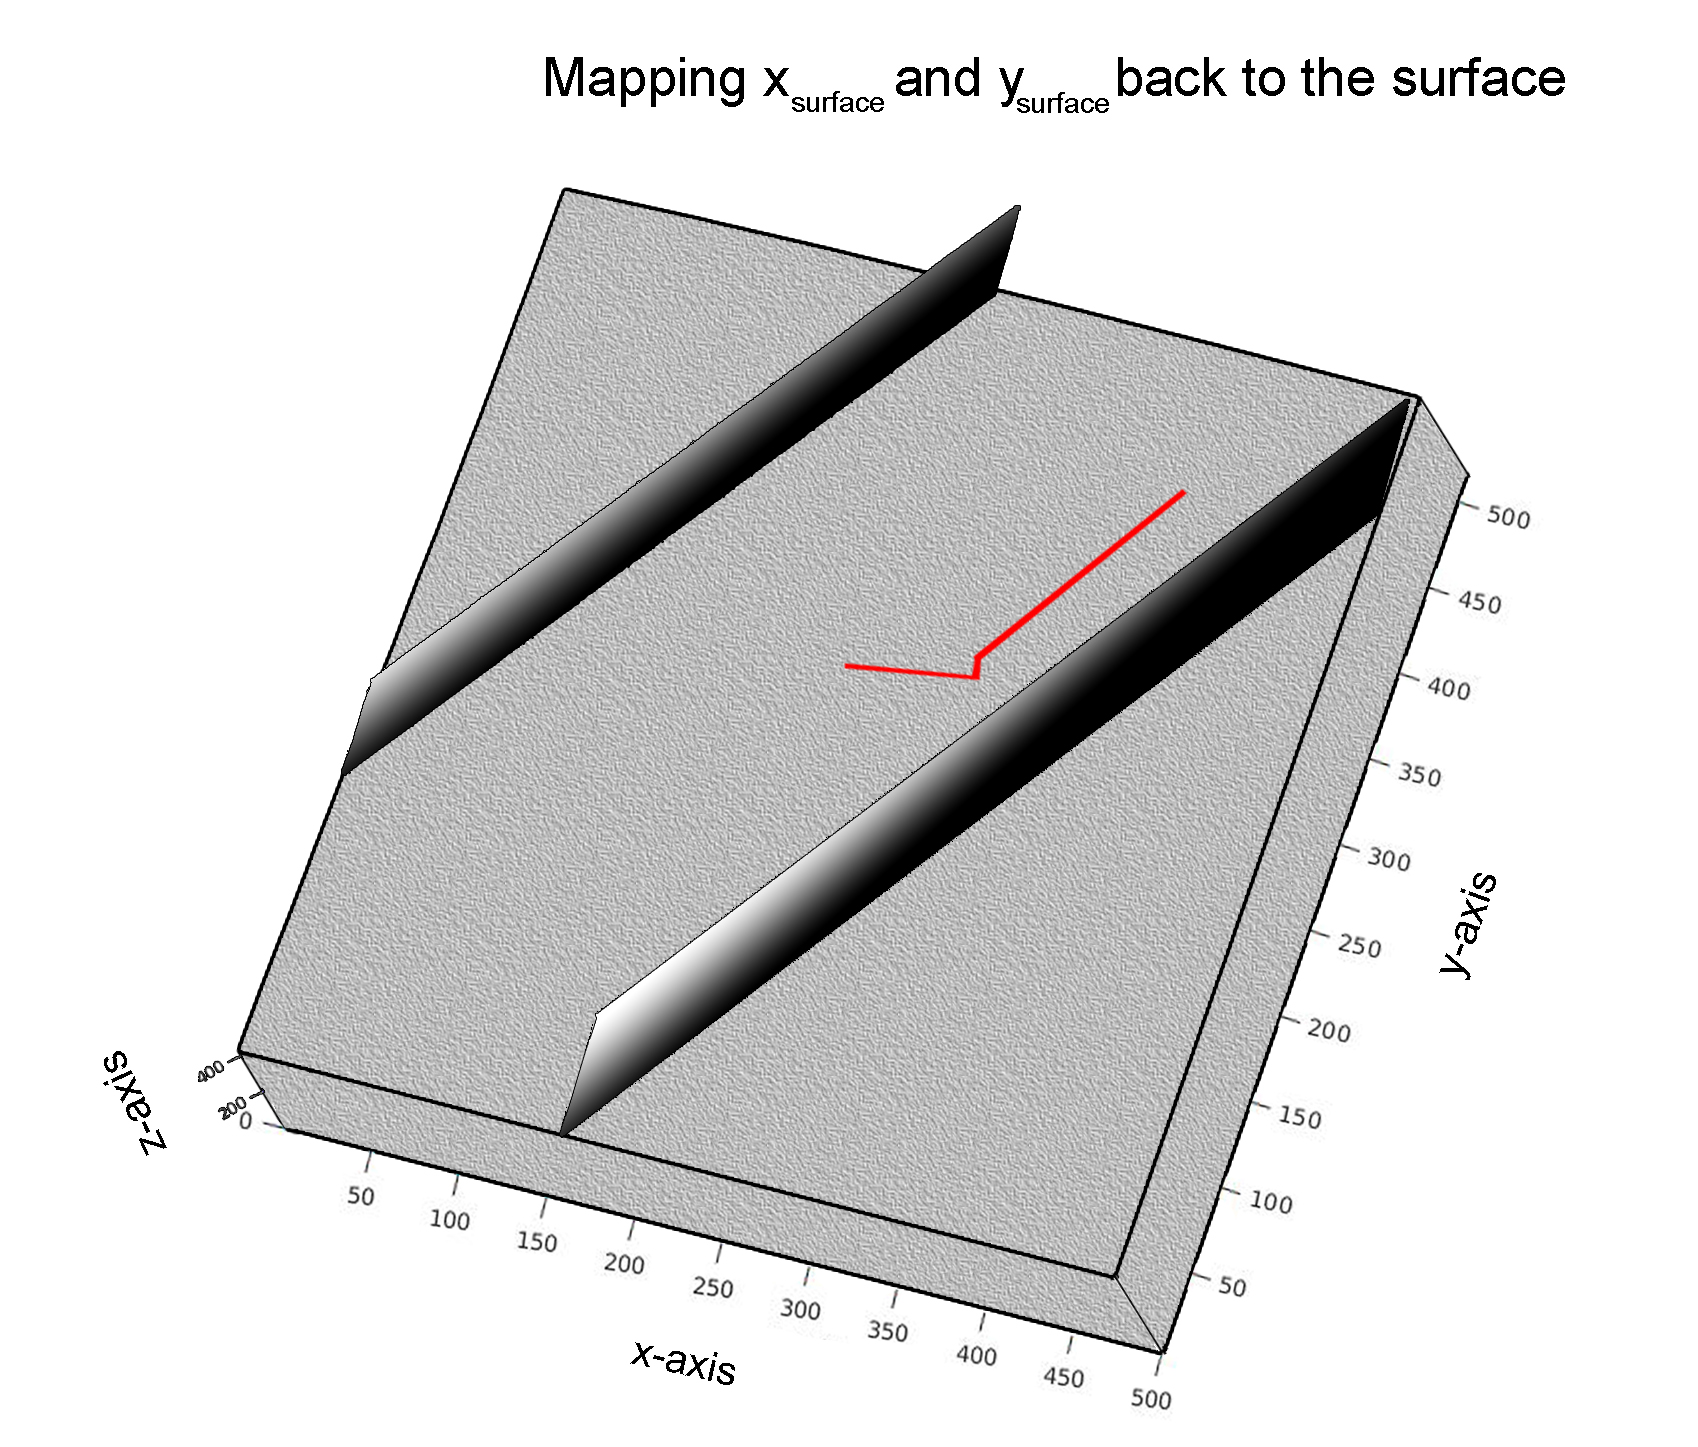
\includegraphics[width=3.5in]{flatsurf.eps}
    \caption{Spherical robot rolling on a flat surface bounded by straight walls. The path of the contact point between the robot and the surface is shown in red (evolving from the bottom left to the top right).}
    \label{fig:flatsurf3D}
\end{figure}

\begin{figure}
\centering
    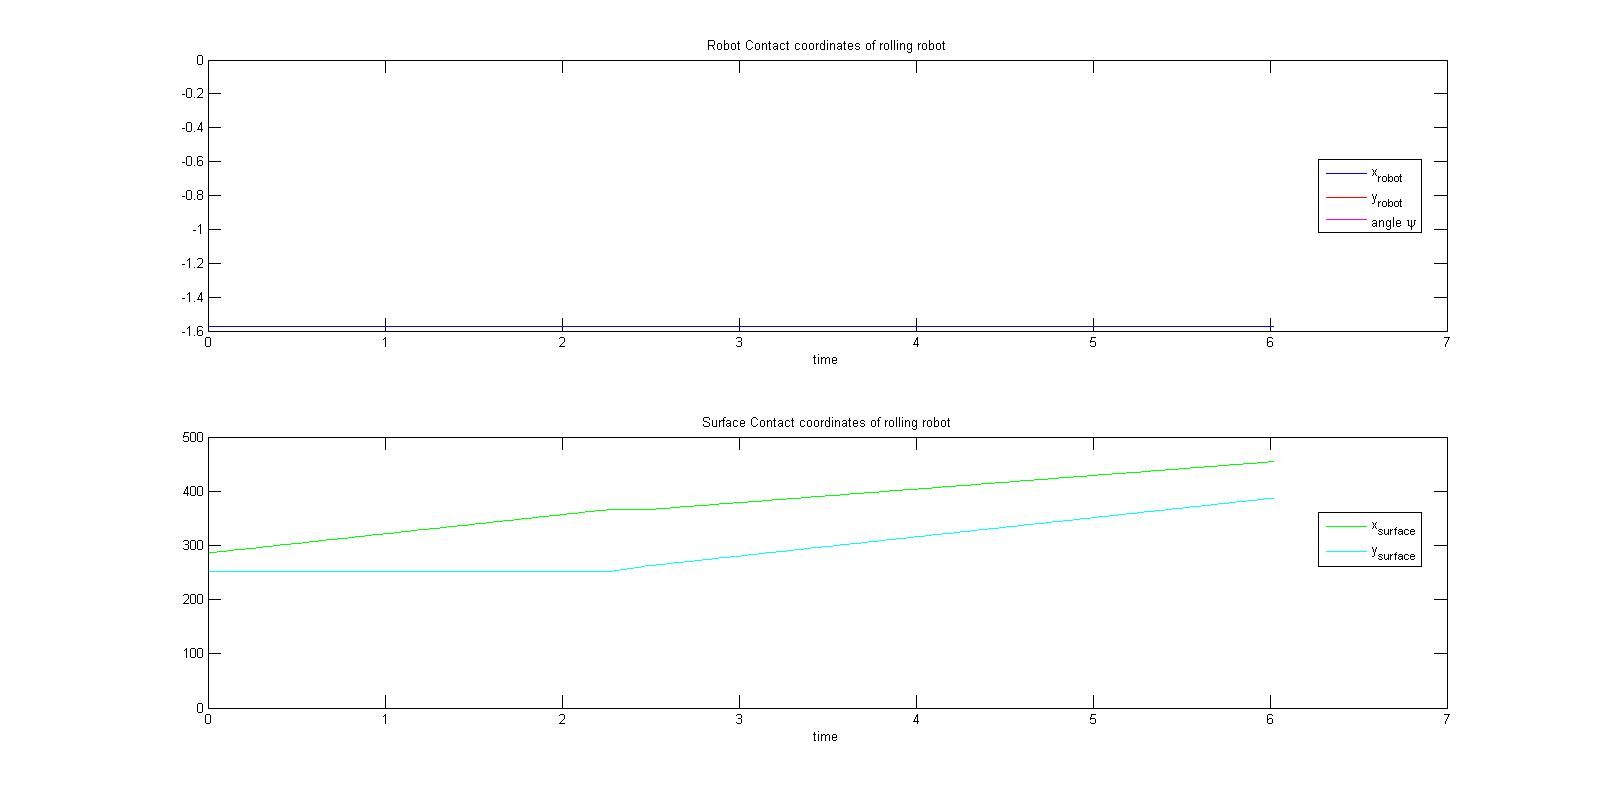
\includegraphics[width=3.5in]{tiltedplane_2D.eps}
    \caption{Evolution of the contact coordinates as a function of time. The robot is rolling on a tilted surface bounded by straight walls (see figure 5).}
    \label{fig:tiltedplane2D}
\end{figure}
\begin{figure}
\centering
    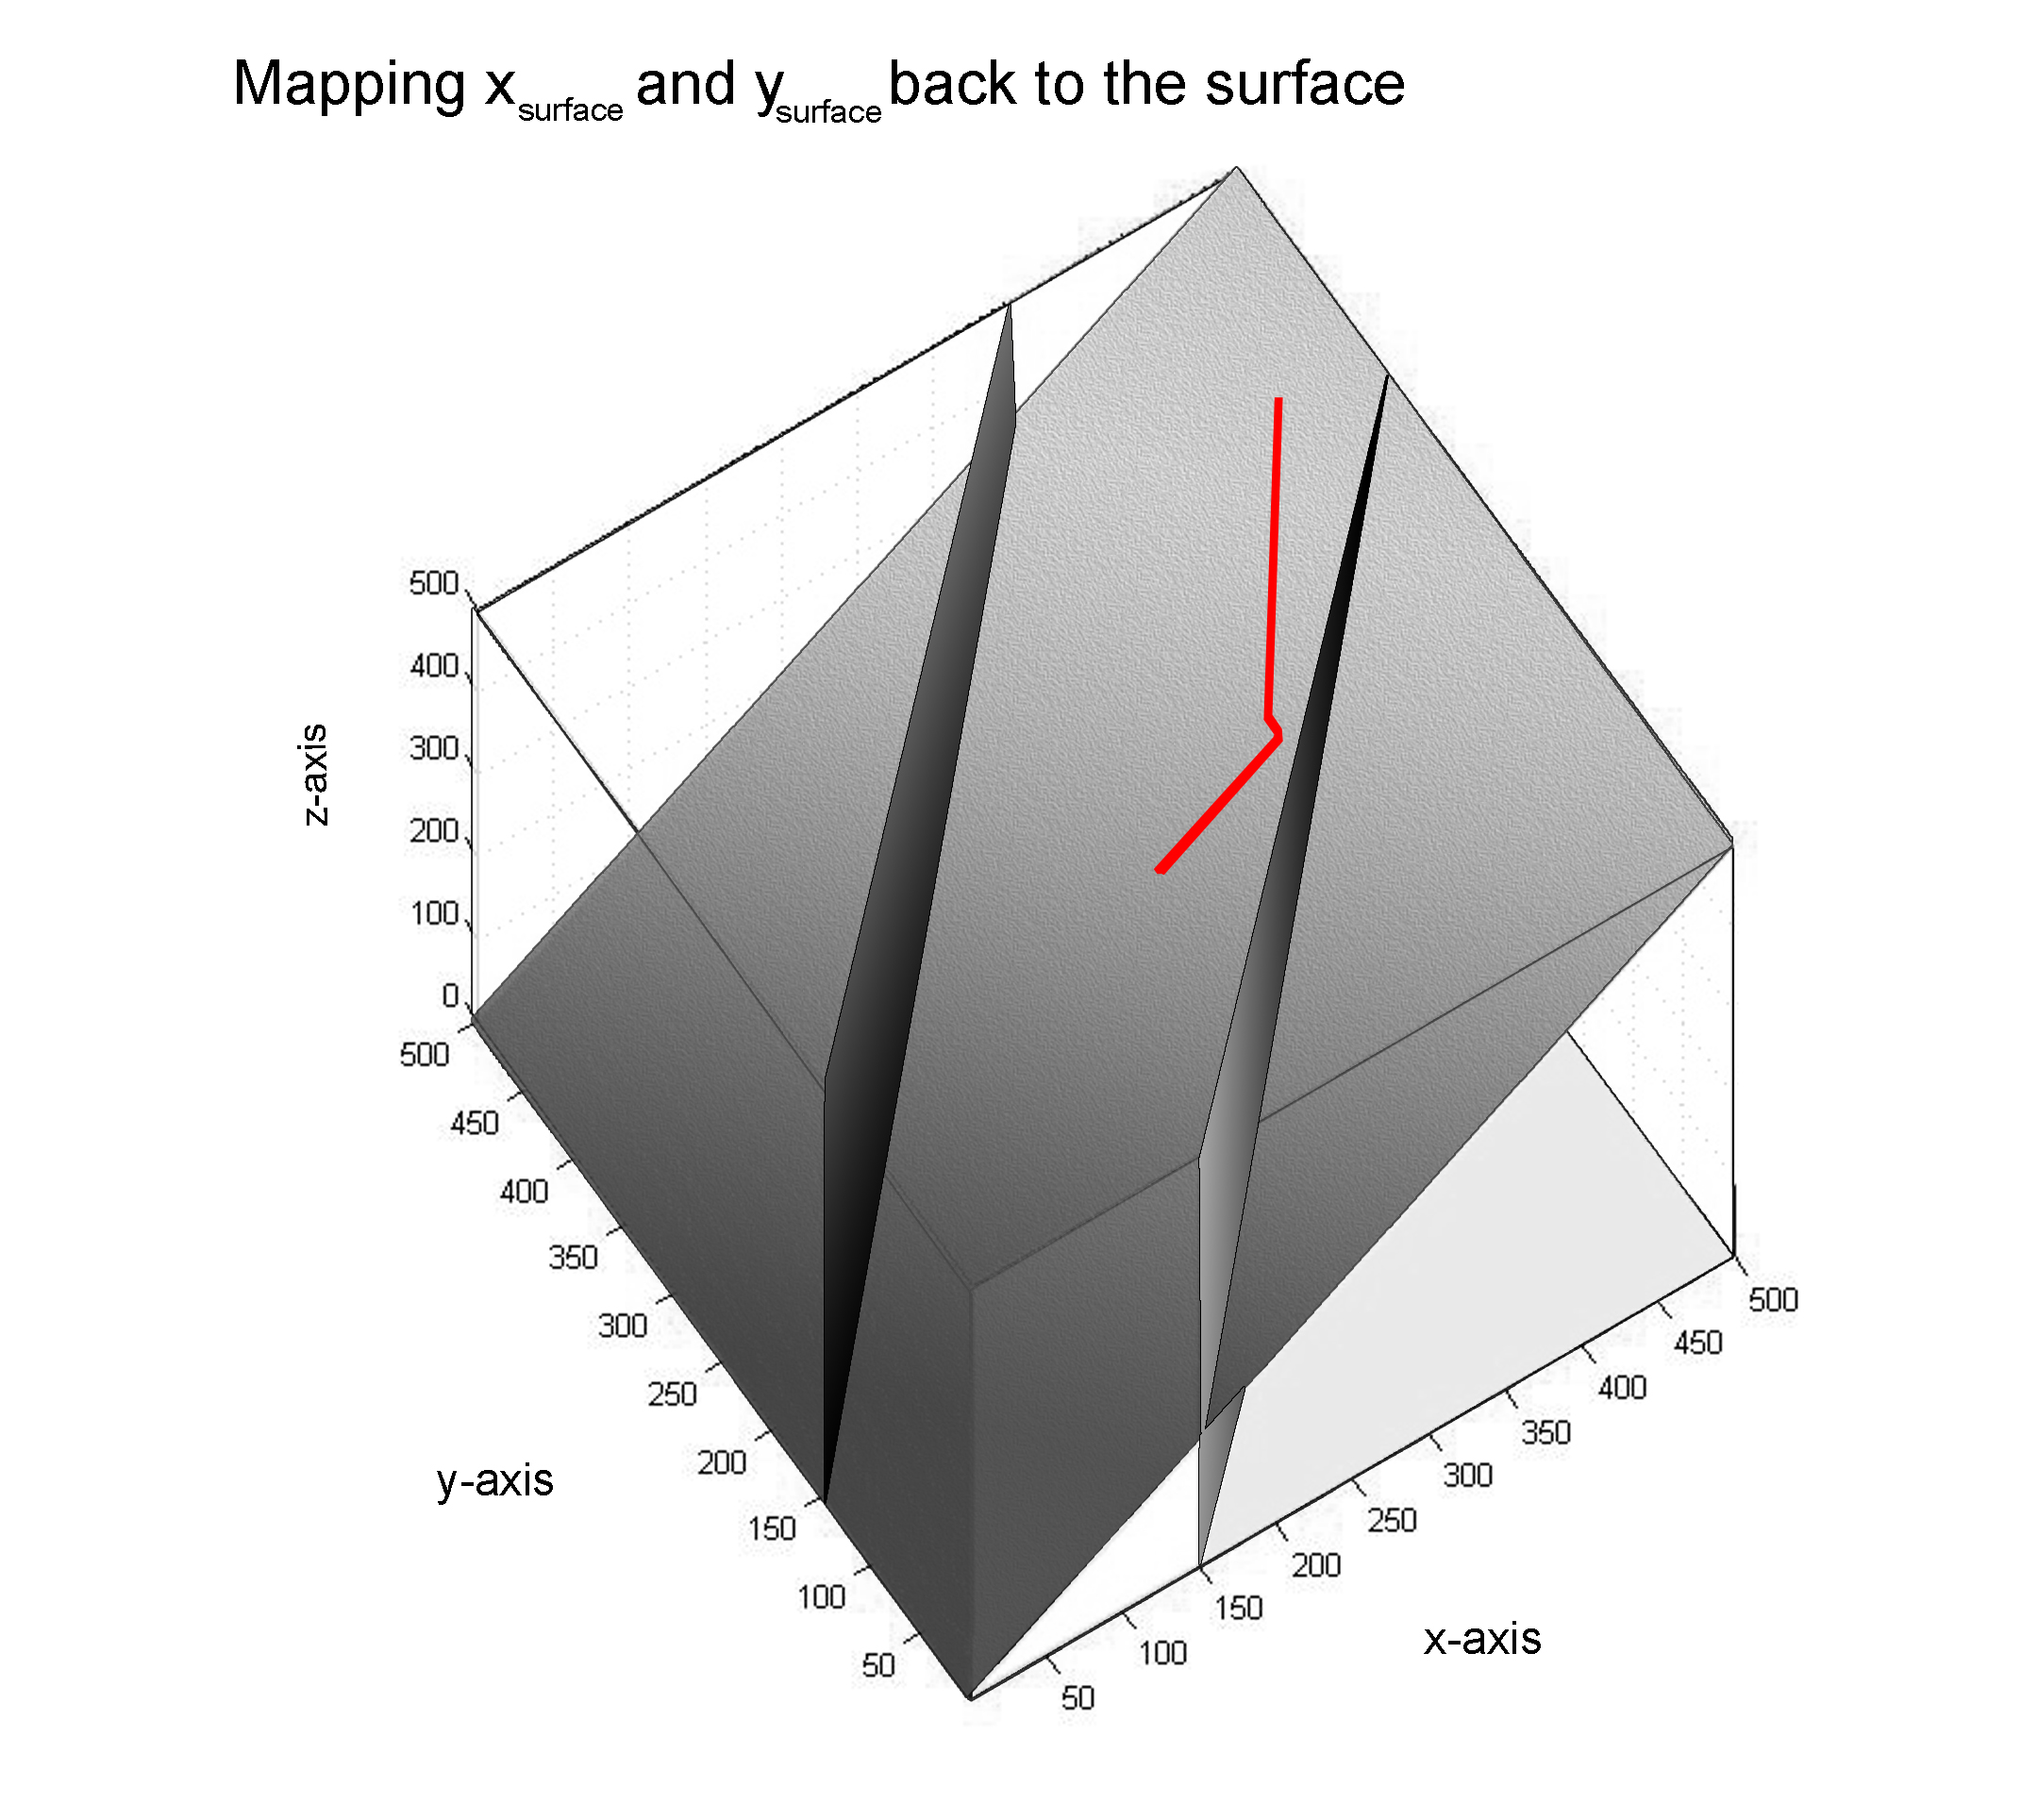
\includegraphics[width=3.5in]{tiltedplane.eps}
    \caption{Spherical robot rolling on a tilted surface bounded by straight walls. The path of the contact point between the robot and the surface is shown in red (evolving from the bottom left to the top right).}
    \label{fig:tiltedplane3D}
\end{figure}

\begin{figure}
\centering
    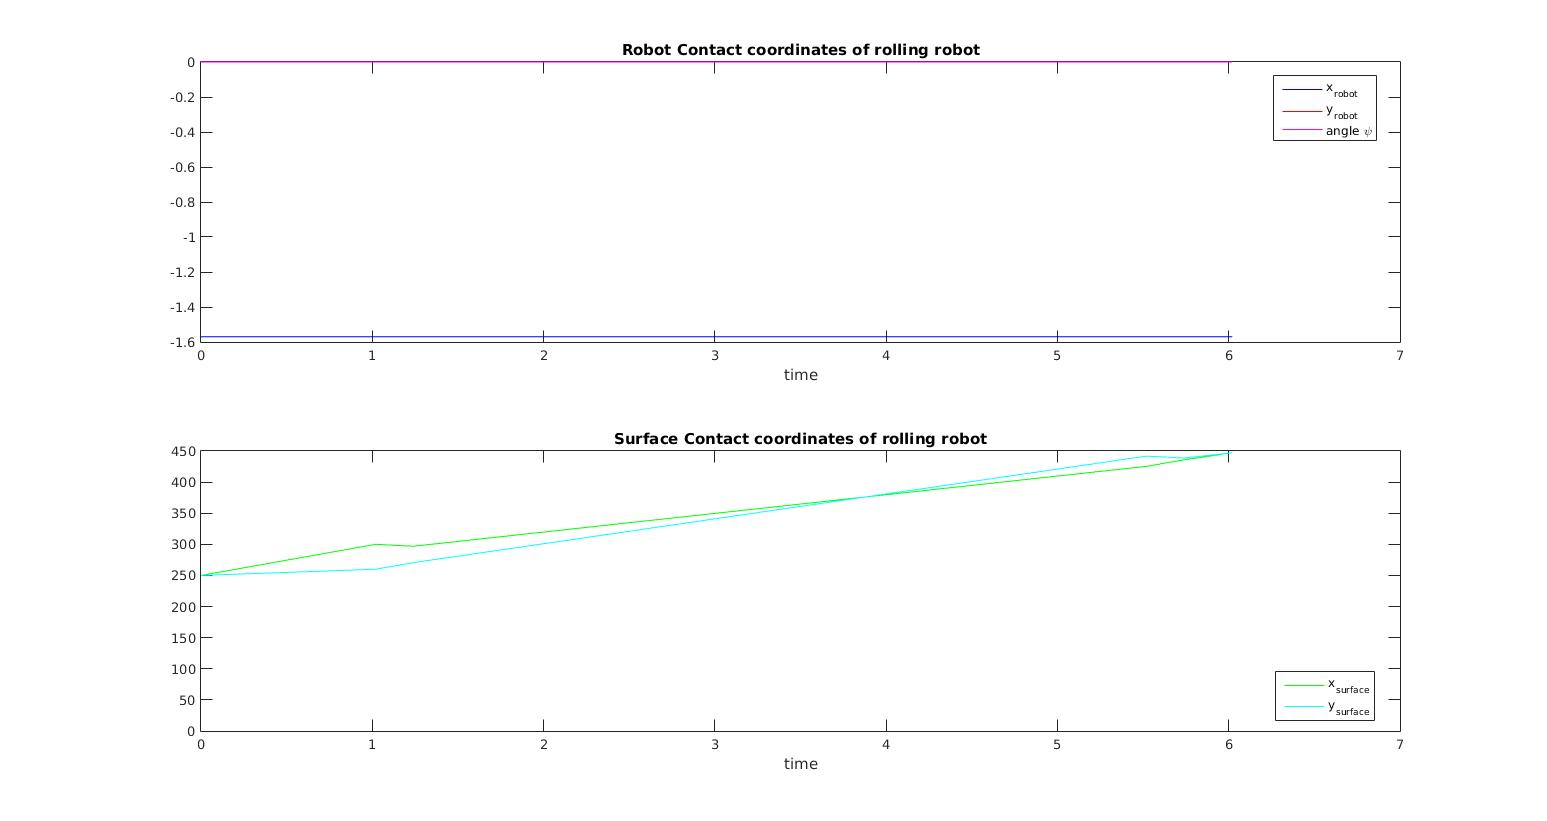
\includegraphics[width=3.5in]{tiltedsines_2D.eps}
    \caption{Evolution of the contact coordinates as a function of time. The robot is rolling on a flat surface bounded by curvy walls in the shape of sine waves (see figure 7).}
    \label{fig:tiltedsines2D}
\end{figure}
\begin{figure}
\centering
    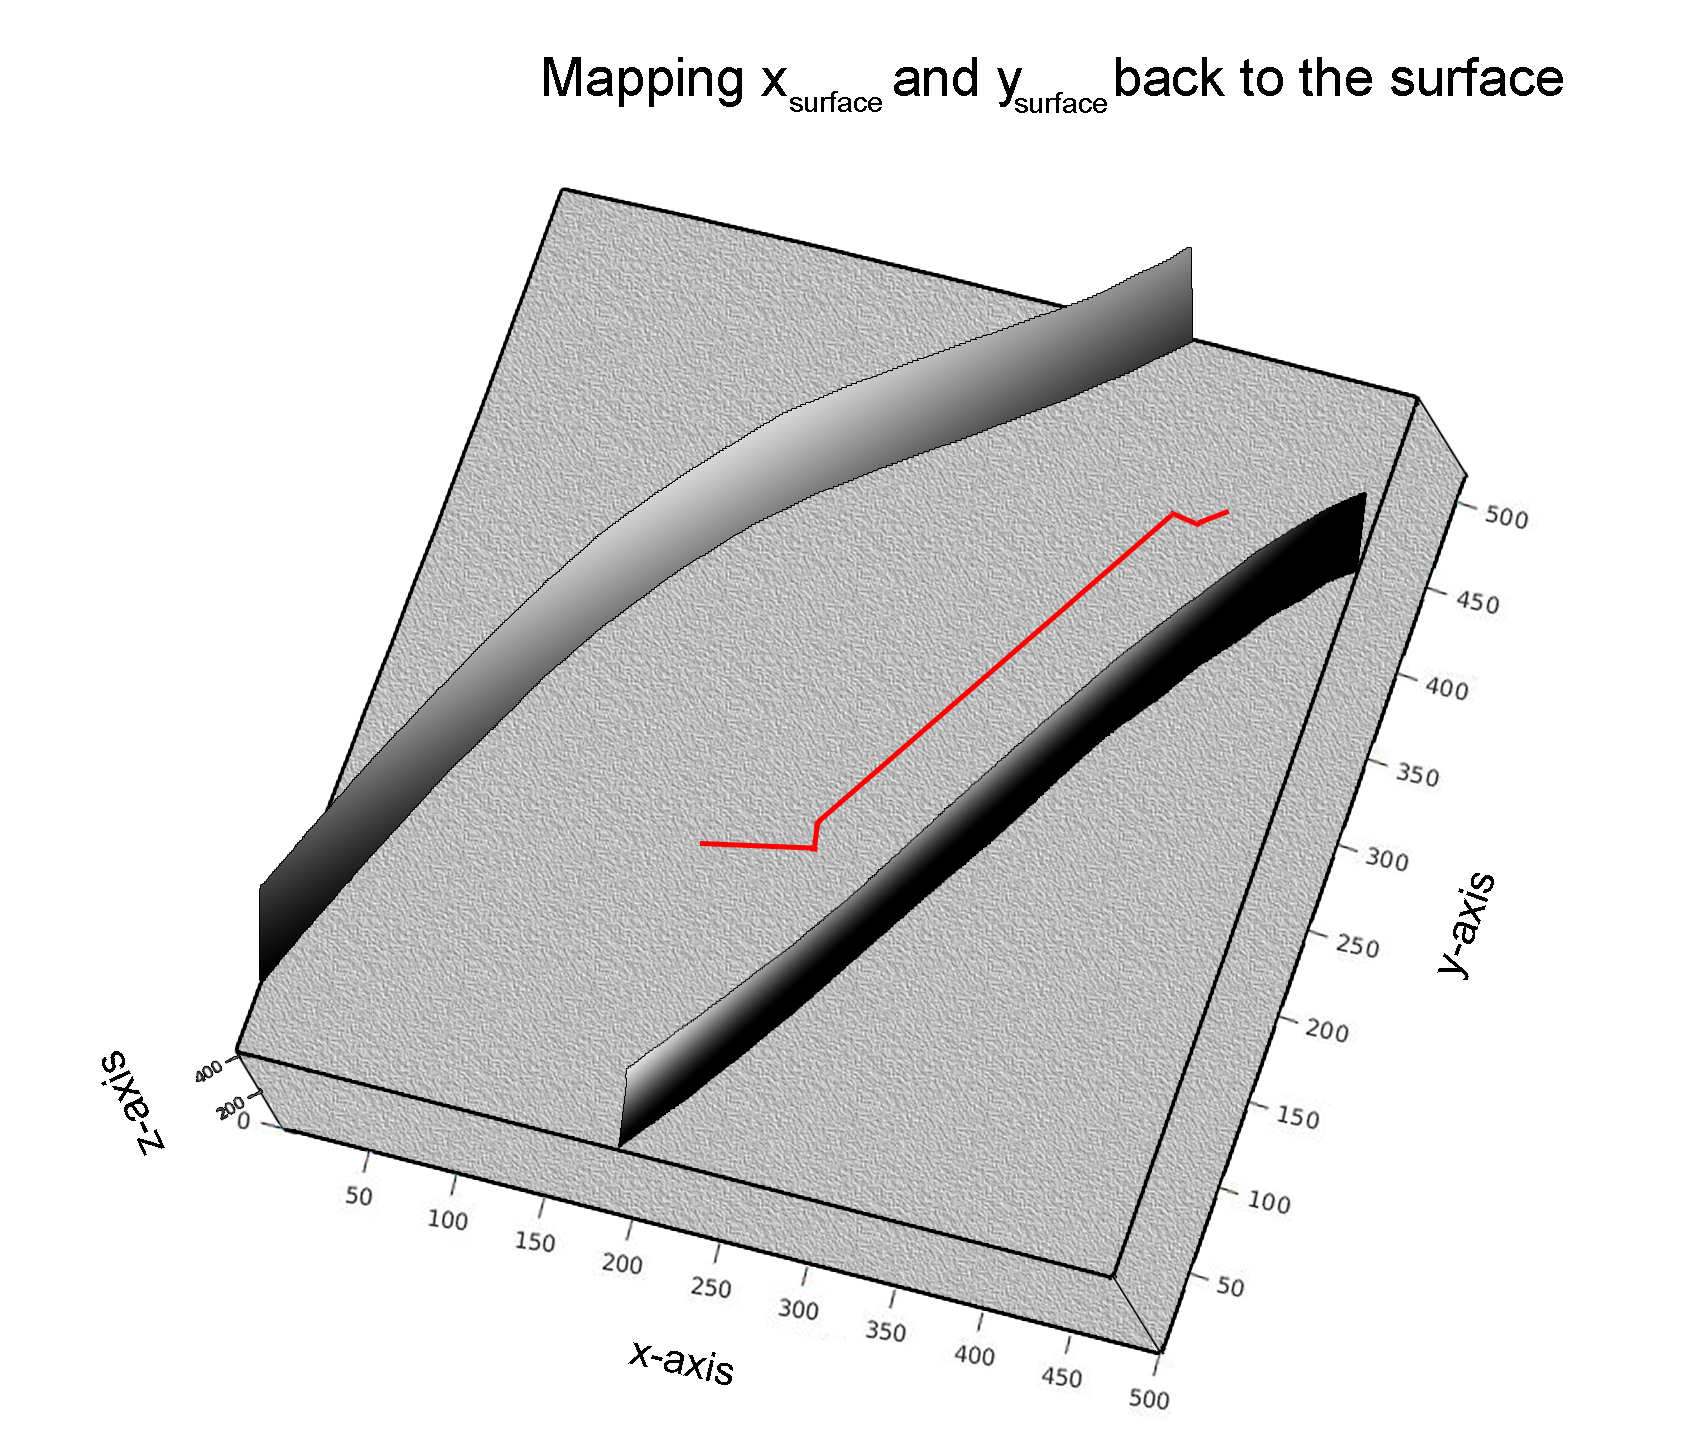
\includegraphics[width=3.5in]{tiltedsines.eps}
    \caption{Spherical robot rolling on a flat surface bounded by curvy walls in the shape of sine waves. The path of the contact point between the robot and the surface is shown in red (evolving from the bottom left to the top right).}
    \label{fig:tiltedsines3D}
\end{figure}

\begin{figure}
\centering
    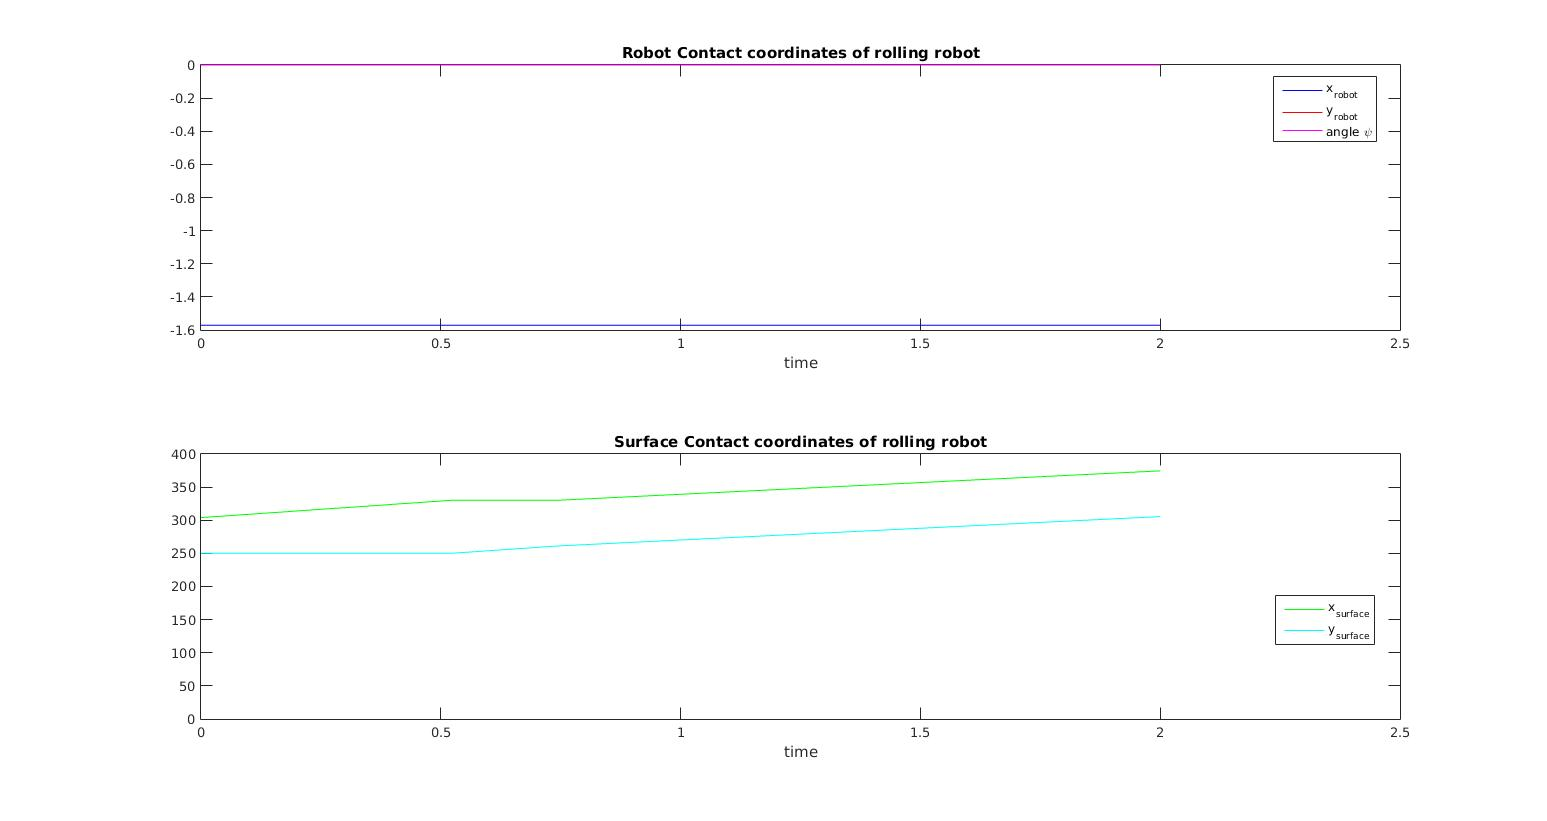
\includegraphics[width=3.5in]{sinewave_2D.eps}
    \caption{Evolution of the contact coordinates as a function of time. The robot is rolling on a curved surface, in the shape of a sine wave, bounded by straight walls (see figure 9).}
    \label{fig:sinewave2D}
\end{figure}
\begin{figure}
\centering
    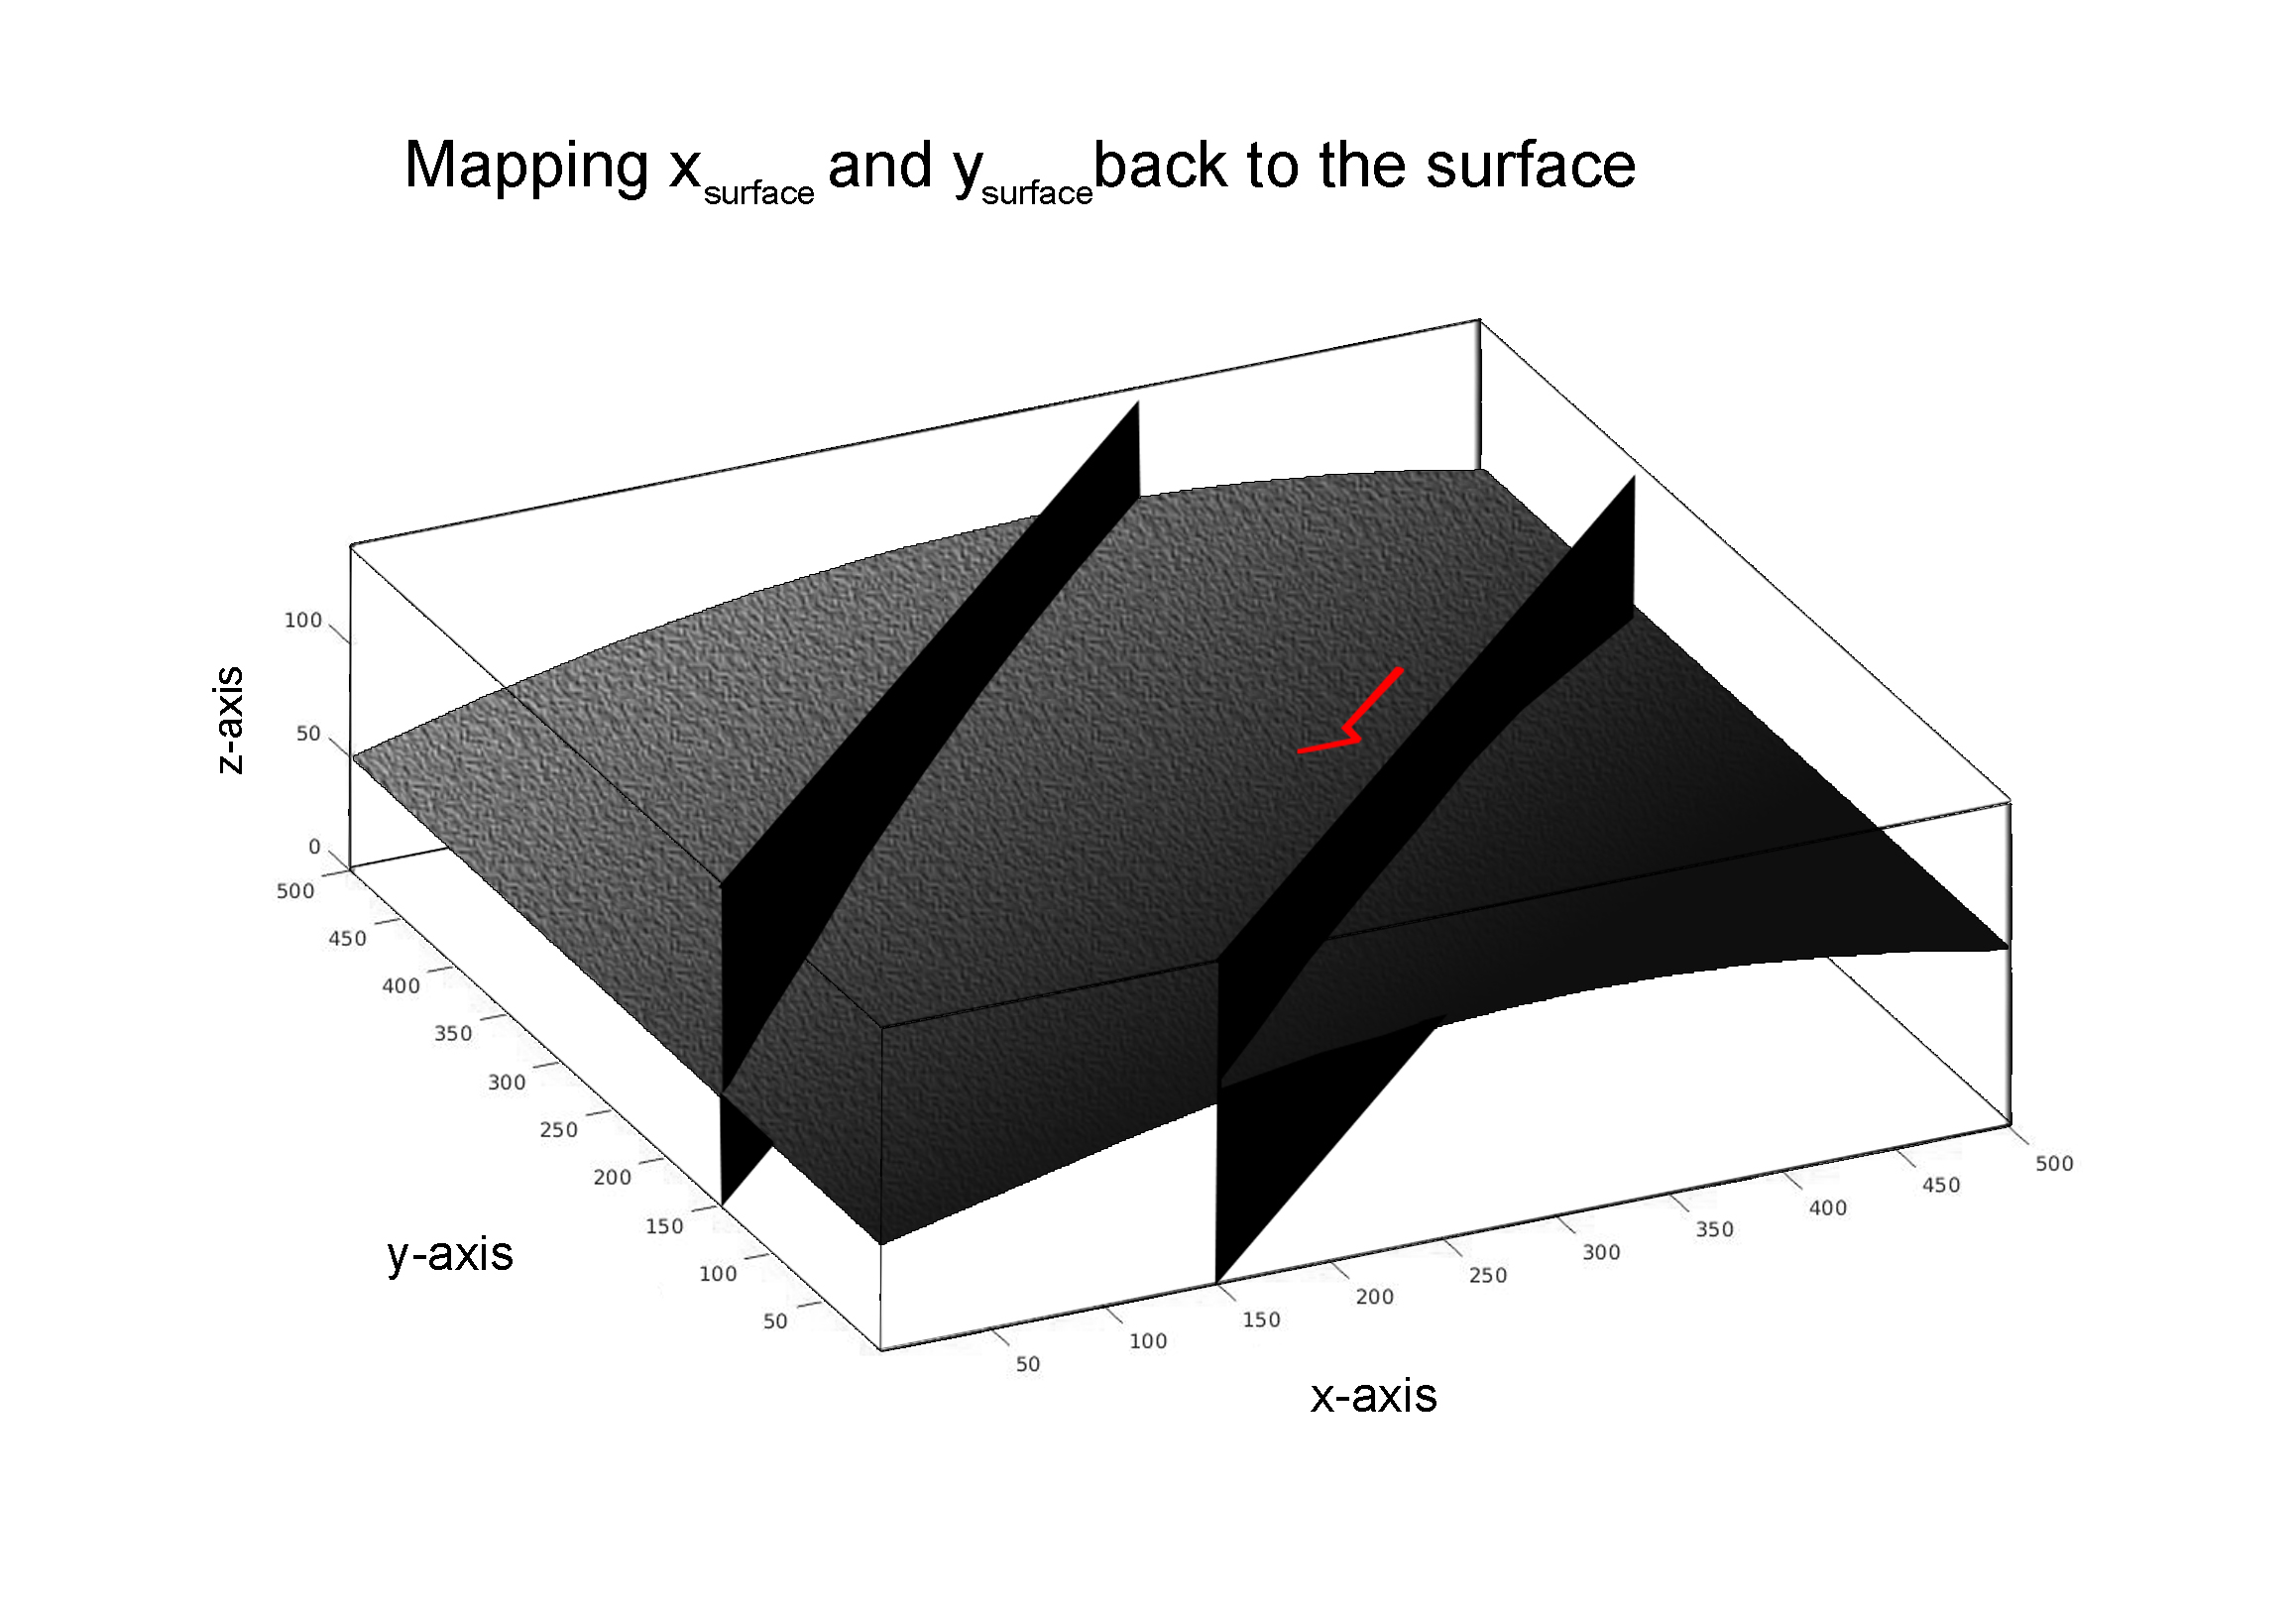
\includegraphics[width=3.5in]{sinewave.eps}
    \caption{Spherical robot rolling on a curved surface, in the shape of a sine wave, bounded by straight walls. The path of the contact point between the robot and the surface is shown in red (evolving from the bottom left to the top right).}
    \label{fig:sinewave3D}
\end{figure}

%Here we need to put a description of the motion, figures, etc. and provide a discussion of these figures.
We now present some example results of our algorithm when applied to a spherical robot rolling on a few simple surfaces with boundaries. As shown in figures 2 through 9 our code can model a spherical robot successfully rolling on a flat surface bounded by straight and curvy walls as well as rolling on tilted surfaces and curved ones. See section IV-F for examples of boundaries and surfaces already implemented in our code. From this knowledge, we are able to simulate path planning on any arbitrary 3D surface.

Figure 2 shows the evolution of the contact variables as a function of time. Those contact variables correspond to the local coordinate chart C defined in Table 1 where the top plot refers to the spherical robot and the bottom plot refers to the plane. Also in the top plot we have the angle of contact $\psi$ defined in Table 1. Figure 3 shows the mapping of those contact variables onto $\mathbb{R}^3$ via our local coordinate charts. As we can see, the robot bounces and reorientates, thus reducing the number of bounces it would make otherwise. Figures 4 and 5 are a similar example when tilting the surface, figures 6 and 7 show the robot on a flat surface with curvy walls and for figures 8 and 9 curvature on our surface was added.

Due to our discretization of the spherical robot into a three dimensional cubic matrix it is very difficult to ensure that there is only one contact point between the robot and the surface at each step of the algorithm (this is a key assumption in the mathematical derivation of our model). Thus, our best results are found when dealing with 3D surfaces that have minimal curvature. When curvature is increased, we suspect that significantly decreasing our discretization step should help. However, we are not able to quantify this due to lack of computer memory. Indeed, reducing the discretization step in our matrices amounts to increasing memory usage cubically.

Finally, this model could be further used to generate a rough map of both the surface and the boundary. Since it is already computing the tangent planes at the contact points, it is not much more difficult to adapt the code for such a task.

\section{Conclusion} 
Instead of being guided by a camera or a sonar system our robot is primarily guided by contact (rolling or sliding on the surface). The robot bounces off the boundary of the surface thus providing information about the shape of the wall. To describe the bouncing of the robot we simply use Snell's Law. The information provided by the location of the contact point between the robot and the surface as well as the way the robot bounces off the walls can be used to both re-orientate the robot and better guide it as well as partially map the boundaries of the surface so that if, for instance, a second robot was following the first one its trajectory could be optimized and it would not need to hit any of the boundaries to go through the tunnel. 
In comparison, Akhtar et al. \cite{Akhtar15}, who used car-like robots, experienced calibration errors when observing the closed-loop performance and had to pay an unneeded amount of attention to the alignment of the wheels. These issues are avoidable when using a spherical robot. Finally, by letting the robot choose a not necessarily smooth path, the design would be more cost effective. Indeed, according to Yang et al. \cite{Yang15}, it is more cost effective to not put as much effort into generating smooth paths since they `introduce external local controls for generating paths'. The dynamics of contact of the robot with the boundary can also be used to quantify the stiffness of the boundary. Pressure sensing has not been treated in this paper.

\appendices
\section{Kinematics derivations}
In this section we summarize some of the derivations in this paper, relying heavily on references from (\cite{book}, Chapter 5), and \cite{DJMontana}. 

In these calculations we assume that the relative curvature is locally invertible.  Singular relative curvature will allow small motions of the object while causing large motions of the contact, thus resulting in loss of continuity.  The contact frames $ C_0 $ and $ C_f $ are the coordinate frames that agree with the normalized Gauss frames induced by the coordinate charts $ (c_0, U_0) $ and $ (c_f, U_f) $ at the points of contact $ p_0 (t) $ and $ p_f(t) $. The local frames are the coordinate frames that are fixed relative to frames $ O $ and $ F $, and which agree with the normalized Gauss frames at the points of contact. If $ (\omega_x, \omega_y) $ are the rolling velocities along the tangent plane at the point of contact, $ \omega_z $ is the rotational velocity about the contact normal, and $ (v_x, v_y,v_z) $ are the linear velocities along the tangent plane. Since we have pure rolling $ v_x = v_y = 0 $ and $ \omega_z =0 $. 

Using the fact that the body velocity of the contact frame $C $ relative to the reference frame $ O $ of the object is given in terms of the fundamental forms of the surface $ (M_p, K_p, T_p ) $ relative to the coordinate chart of the surface $ (c_f, U_f) $ by (\cite{book}, Lemma 5.10), we have:
\begin{center}
Equations 6:
\end{center}

\begin{align*}
v_{oc} &= \begin{bmatrix}
	   M\dot{\alpha} \\
	   0
	 \end{bmatrix} \\
\end{align*}
\begin{center}
and
\end{center}

\begin{align*}
\hat{w}_{oc} &= \begin{bmatrix}
						0 & -\omega_z & \omega_y \\
						\omega_z & 0 & -\omega_x \\
						-\omega_y & \omega_x & 0
					\end{bmatrix} \\
	     &= 	\left[\begin{array}{c|c}
											\begin{array}{cc}
												0 & -TM\dot{\alpha} \\
												TM\dot{\alpha} & 0 
											\end{array}				& KM\dot{\alpha} \\ \cline{1-2}	
											-(KM\dot{\alpha})^T & 0
										\end{array}\right]. \\ \\
\end{align*}
Relating the spatial and body velocities by a similarity transformation $ R_\psi $, each of the quantities in the equation of motion can be expressed in terms of geometric and motion parameters as:
\begin{center}
Equations 7:
\end{center}


\vspace{0.4cm}
$\begin{array}{c c}
\left[
\begin{array}{c}
\dot{u_f}\\
\dot{v_f}\\
\end{array}
\right] =
 M_f^{-1}(K_f + R_{\psi} K_o R_{\psi})^{-1}\bigg(
\left[
\begin{array}{c}
-\omega_y\\
\omega_x\\
\end{array}
\right] \\
- R_{\psi} K_o R_{\psi}
\left[
\begin{array}{c}
v_x\\
v_y\\
\end{array}
\right]\bigg)&\\
\end{array}
$
\vspace{0.4cm}

$\begin{array}{c c}
\left[
\begin{array}{c}
\dot{u_o}\\
\dot{v_o}\\
\end{array}
\right]
= M_o^{-1}R_{\psi}(K_f + R_{\psi} K_o R_{\psi})^{-1}\bigg(
\left[
\begin{array}{c}
-\omega_y\\
\omega_x\\
\end{array}
\right] &\\
+  K_f
\left[
\begin{array}{c}
v_x\\
v_y\\
\end{array}
\right]\bigg)&
\end{array}$
\vspace{0.4cm}


$\dot{\psi} = \omega_z + T_f M_f 
\left[
\begin{array}{c}
\dot{u_f}\\
\dot{u_f}\\
\end{array}
\right]
+ T_o M_o
\left[
\begin{array}{c}
\dot{u_o}\\
\dot{v_o}\\
\end{array}
\right]$


%\href{https://github.com/cbenn/guidancerobotics}{code}

% use section* for acknowledgment
\section*{Acknowledgment}
This research was supported by the EPSCoR Office at the University of Wyoming. The researchers gratefully acknowledge this support.


\newpage

\bibliographystyle{IEEEtran}
\bibliography{IEEEabrv,references.bib}

%\begin{thebibliography}{1}
%
% \bibliography{IEEEabrv,references.bib}
%
%
%\bibitem{IEEEhowto:kopka}
%H.~Kopka and P.~W. Daly, \emph{A Guide to \LaTeX}, 3rd~ed.\hskip 1em plus
%  0.5em minus 0.4em\relax Harlow, England: Addison-Wesley, 1999.
%
%\end{thebibliography}

%\bibliography{references.bib}
%\bibliographystyle{ieeetr}


%\begin{IEEEbiography}{Thomas Rochais}
%Biography text here.
%\end{IEEEbiography}

% if you will not have a photo at all:
%\begin{IEEEbiography}{Courtney Sheyko}
%Biography text here.
%\end{IEEEbiography}

% insert where needed to balance the two columns on the last page with
% biographies
%\newpage

%\begin{IEEEbiography}{Farhad Jafari}
%Farhad Jafari, Professor of Mathematics mathematical interests include functional analysis and operator theory, semigroup theory, harmonic analysis, moment problems, and control theory. He is particularly interested in problems arising from mathematical physics. He serves on the editorial boards of two journals (J. Semigroups Theory and Applications, and Linear and Topological Algebra) and served as the Department Head for 6 years between 2009-2015. Jafari has published over 50 refereed articles.
%\end{IEEEbiography}

\end{document}


